\documentclass[11pt,parskip=full]{scrartcl}%article}
%\setlength{\parskip}{1em}

%%%%%%%%%%%%%%%%%%%%%%
%% PACKAGE INCLUDES %%
%%%%%%%%%%%%%%%%%%%%%%

\usepackage{array}           % For defining \newcolumntype.
\usepackage{amsmath}
\usepackage{amssymb}
\usepackage{amsthm}          % Provides 'proof' environment.
\usepackage[english]{babel}  % For defining 'theorem/corollary/lemma' environments.
\usepackage{bm}              % Provides bold \pi
\usepackage{booktabs}
\usepackage{hyperref}
\usepackage{textcomp}
\usepackage{gensymb}         % Enables \degree command for °C.
\usepackage{todonotes}
\usepackage{subfig}
\usepackage{enumitem}
\usepackage{graphicx}
\usepackage{listings}
\usepackage{mathtools}
\usepackage{listings} % http://ctan.org/pkg/listings

\lstset{
  basicstyle=\ttfamily,
  mathescape
}


%%%%%%%%%%%%%%%%%
%% STYLE SETUP %%
%%%%%%%%%%%%%%%%%

% Define some custom colors.
\definecolor{mylinkcolor}{RGB}{000, 114, 166}
\definecolor{mycitecolor}{RGB}{255, 154, 071}
\definecolor{myurlcolor}{RGB}{000, 114, 166}

% Set itemize format.
\setitemize{noitemsep,topsep=-5pt,parsep=5pt,partopsep=0pt}

% Define column types that allow fixed width params.
\newcolumntype{L}[1]{>{\raggedright\let\newline\\\arraybackslash\hspace{0pt}}m{#1}}
\newcolumntype{C}[1]{>{\centering\let\newline\\\arraybackslash\hspace{0pt}}m{#1}}
\newcolumntype{R}[1]{>{\raggedleft\let\newline\\\arraybackslash\hspace{0pt}}m{#1}}

% Color setup for hyperlinks/references/citations/urls.
\hypersetup{
    colorlinks,
    linkcolor={mylinkcolor},
    citecolor={mycitecolor},
    urlcolor={myurlcolor}
}

% Specify hyphenation of words on line break.
\hyphenation{Figure Table Chapter Section}

\long\def\/*#1*/{}



%%%%%%%%%%%%
%% MACROS %%
%%%%%%%%%%%%

% Set default font family to sans-serif.
\renewcommand*{\familydefault}{\sfdefault}
\newcommand{\Tau}{\mathrm{T}}

\newcommand*{\ie}{i.e., }
\newcommand*{\eg}{e.g., }
\newcommand*{\wrt}{w.r.t. }

\newcommand*{\tokens}{\mathcal{T}}          % Set of tokens.
\newcommand*{\orders}{\mathcal{O}}          % Set of orders.
\newcommand*{\itokens}{\mathcal{I}^t}       % Set of token indices.
\newcommand*{\itokenpairs}{\mathcal{I}^p}   % Set of token index pairs.
\newcommand*{\iorders}{\mathcal{I}^o}       % Set of order indices.
\newcommand*{\ibuyorders}{\mathcal{I}^b}    % Set of buy order indices.
\newcommand*{\isellorders}{\mathcal{I}^s}   % Set of sell order indices.

% Macros for references etc.
\newcommand*{\figref}[1]{\hyperref[{#1}]{Figure~\ref*{#1}}}
\newcommand*{\tabref}[1]{\hyperref[{#1}]{Table~\ref*{#1}}}
\newcommand*{\secref}[1]{\hyperref[{#1}]{Section~\ref*{#1}}}
\newcommand*{\subsecref}[1]{\hyperref[{#1}]{Section~\ref*{#1}}}
\newcommand*{\thmref}[1]{\hyperref[{#1}]{Theorem~\ref*{#1}}}
\newcommand*{\crlref}[1]{\hyperref[{#1}]{Corollary~\ref*{#1}}}
\newcommand*{\lemref}[1]{\hyperref[{#1}]{Lemma~\ref*{#1}}}

% Macros for theorems|corollaries|lemmas.
\newtheorem{theorem}{Theorem}[section]
\newtheorem{corollary}{Corollary}[theorem]
\newtheorem{lemma}[theorem]{Lemma}

%Notational abbreviations

\def\pO{\mathcal{O}}
\def\ra{\rightarrow}

\newcommand*{\erc}{ERC20 }
%%%%%%%%%%%%%%
%% DOCUMENT %%
%%%%%%%%%%%%%%

\title{
  Multi-token Batch Auctions with Uniform Clearing Prices on Plasma\\
  - \\
  \Large Specification For Implementation}
\author{Gnosis}

\date{\today}



\begin{document}

\maketitle


\begin{abstract}

This document outlines a formal specification of a batch auction exchange of ERC20 tokens using the plasma technologies. 
The batch auction mechanism will enable the execution of ring trades between different tokens. 
Plasma technologies will provide the same security for users as if the tokens were held in the ethereum blockchain. 
But gas costs will be significantly reduced due to the off-chain nature of the exchange mechanism. 
It is recommended for the reader to familiarize themselves with Plasma\cite{plasma}, Plasma MVP\cite{MVP}, snarks\cite{snarks} and batch auctions\cite{batch} before reading this spec. 

\end{abstract}

\tableofcontents

\newpage
\section{Introduction}
\label{sec:introduction}

\paragraph{Multi-batch auctions with uniform clearing prices}

This specification outlines a trading mechanism between several \erc tokens. Each batch accepts orders to buy any \erc token with any other \erc token for a maximal specified limit price. All orders are collected over some time interval and then an \emph{uniform clearing price} over all token pairs is calculated. 

For a list of $k$ trading tokens denoted by $\Tau$ with clearing prices $\{p_{ij}\}$, we call the set of prices $\{p_{ij}| \tau_i, \tau_j \in \Tau\}$ an uniform clearing price, if
\begin{align} \label{arbitrage_free}
  p_{ij} \cdot p_{jk} &= p_{ik}\\
  p_{ij} &= p_{ji}^{-1}
\end{align}


Finding the uniform clearing prices, which also maximize trading volume or other predefined metrics is a complicated task. The paper \cite{priceOptimization} describes a mechanism in detail. Uniform clearing prices are beneficial for any trader since they are arbitrage-free and ensure good liquidity via built-in ring trades. For the purpose of this document, it is assumed that these uniform clearing prices for a multi-batch auction can be efficiently determined. \newline
The multi-token batch mechanism is secured against front-running \footnote{Front-running is when a actor enters into an equity/asset trade with foreknowledge of a transaction which will influence the price} by allowing users to submit encrypted orders into the batch auction. Only after the batch has closed the orders be revealed and then the prices can be computed. 


\paragraph{Plasma minimal viable product}

This paper describes the specification for porting this auction mechanism onto a plasma chain. Plasma chains are a second layer scaling solution for blockchains which allow processing a much higher volume of transactions as the underlying blockchain (a.k.a. \emph{root-chain}) with the same security guarantees\footnote{The same security is actually only given under the assumptions that transactions are not censored on the root chain for a longer period of time, and the plasma clients stay online and validate the plasma chain frequently}. This is the main motivation for implementing such mechanism on a plasma chain as it will result in significantly less costs per trade. Unfortunately, plasma chains have also a disadvantages: They come with burdens in terms of complexity and sometimes usability. We are planning to use Ethereum as the root-chain. 

\paragraph{The trade-flow of a batch auction}  

The batch auction exchange is built on a plasma chain operated by a single entity on top of a root-chain. A single batch auction consists of several phases:
\begin{itemize}
\item[(i)] Encryption Key Generation, 
\item[(ii)] Order Collection, 
\item[(iii)] Double Signing, 
\item[(iv)] Decryption Key Generation,
\item[(v)] Batch Price Calculation,
\item[(vi)] Batch Challenging and 
\item[(vii)] Order Executions. 

\end{itemize}
In brief, a batch will proceed as follows: Users will post encrypted orders to the plasma operator, who will then bundle these orders and commit them by posting a single order-block on the plasma chain. Each client will have to validate the orders of this order-block. Only once they have validated the orders, they may double sign their orders to participate in the current batch. The participation acknowledgment will be compactly represented using a crypto-economic signature aggregation schema. With this construction many data-unavailability problems will be avoided because the orders can be represented on the root-chain using only a bitmap.
Once the bitmap is seen by many parties on the plasma chain, the private key for decrypting the orders will be generated using distributed key generation (DKG). Finally, all the data is available to calculate correct prices from the orders and the batch can be settled. 


\newpage

\section{Detailed specification overview}
\subsection{Setup description}

\subsubsection{Definitions}


%Let us start of with writing down some very basic definitions, which we will use throughout this paper.
In our batch auctions all trading will occur between a fixed set, $\Tau = \{\tau_i\}_{i=1}^n$, of $n$ \erc tokens. The collection of orders for which token $i$ is being sold in exchange for token $j$ will be denoted by $\pO_{i\ra j}$. 

After an auction has been closed and uniform clearing prices have been determined, the price matrix can be represented as an $n\times n$ a matrix 
\[P = \{p_{ij}| \tau_i, \tau_j \in \Tau \}.\]
Due to the equations \ref{arbitrage_free}, it is enough to define the uniform clearing price as an one dimensional vector with respect to a reference token $\tau_1$:
\[p_1 = \{p_{1j}| \tau_i \in \Tau \}.\]

For any order $\sigma \in \pO_{i\ra j}$ we define $\nu_p(\sigma)$ as the volume of an order denominated in token $\tau_i$ at clearing prices $p$.


\subsubsection{Plasma chain setup}
We are following the description of the Plasma Minimal Viable Product\cite{MVP}. 
This means all assets are represented in the plasma chain as unspent transaction outputs (utxo). 
These utxos can be transferred to a new owner by making a transaction, waiting for its inclusion into the plasma chain, validating the chain, waiting for the plasma block to be submitted to the root-chain and then, sending a double-sign message to the receiver. 

Any utxo may be exited at any time, by providing a Merkle proof of the receiving transaction. 
However, if the exit is not valid, then it will be canceled via a challenge process.
The mvp also defines a \emph{exit-request-timeperiod}\label{exit-time}, which is usually set to 7 days. The plasma mvp requires people to be online and validate the chain frequently.
The time difference between two consecutive validations should not be bigger than exit-request-timeperiod.


\subsection{The trade flow}
\label{subsec:data}

In the following section we will describe the general tradeflow through all its phases: Encryption Key generation, Order Collection, Double signing, DKG Private Key Generation, Price submission, Price Proofs and Order Executions.

\begin{figure}
\centering
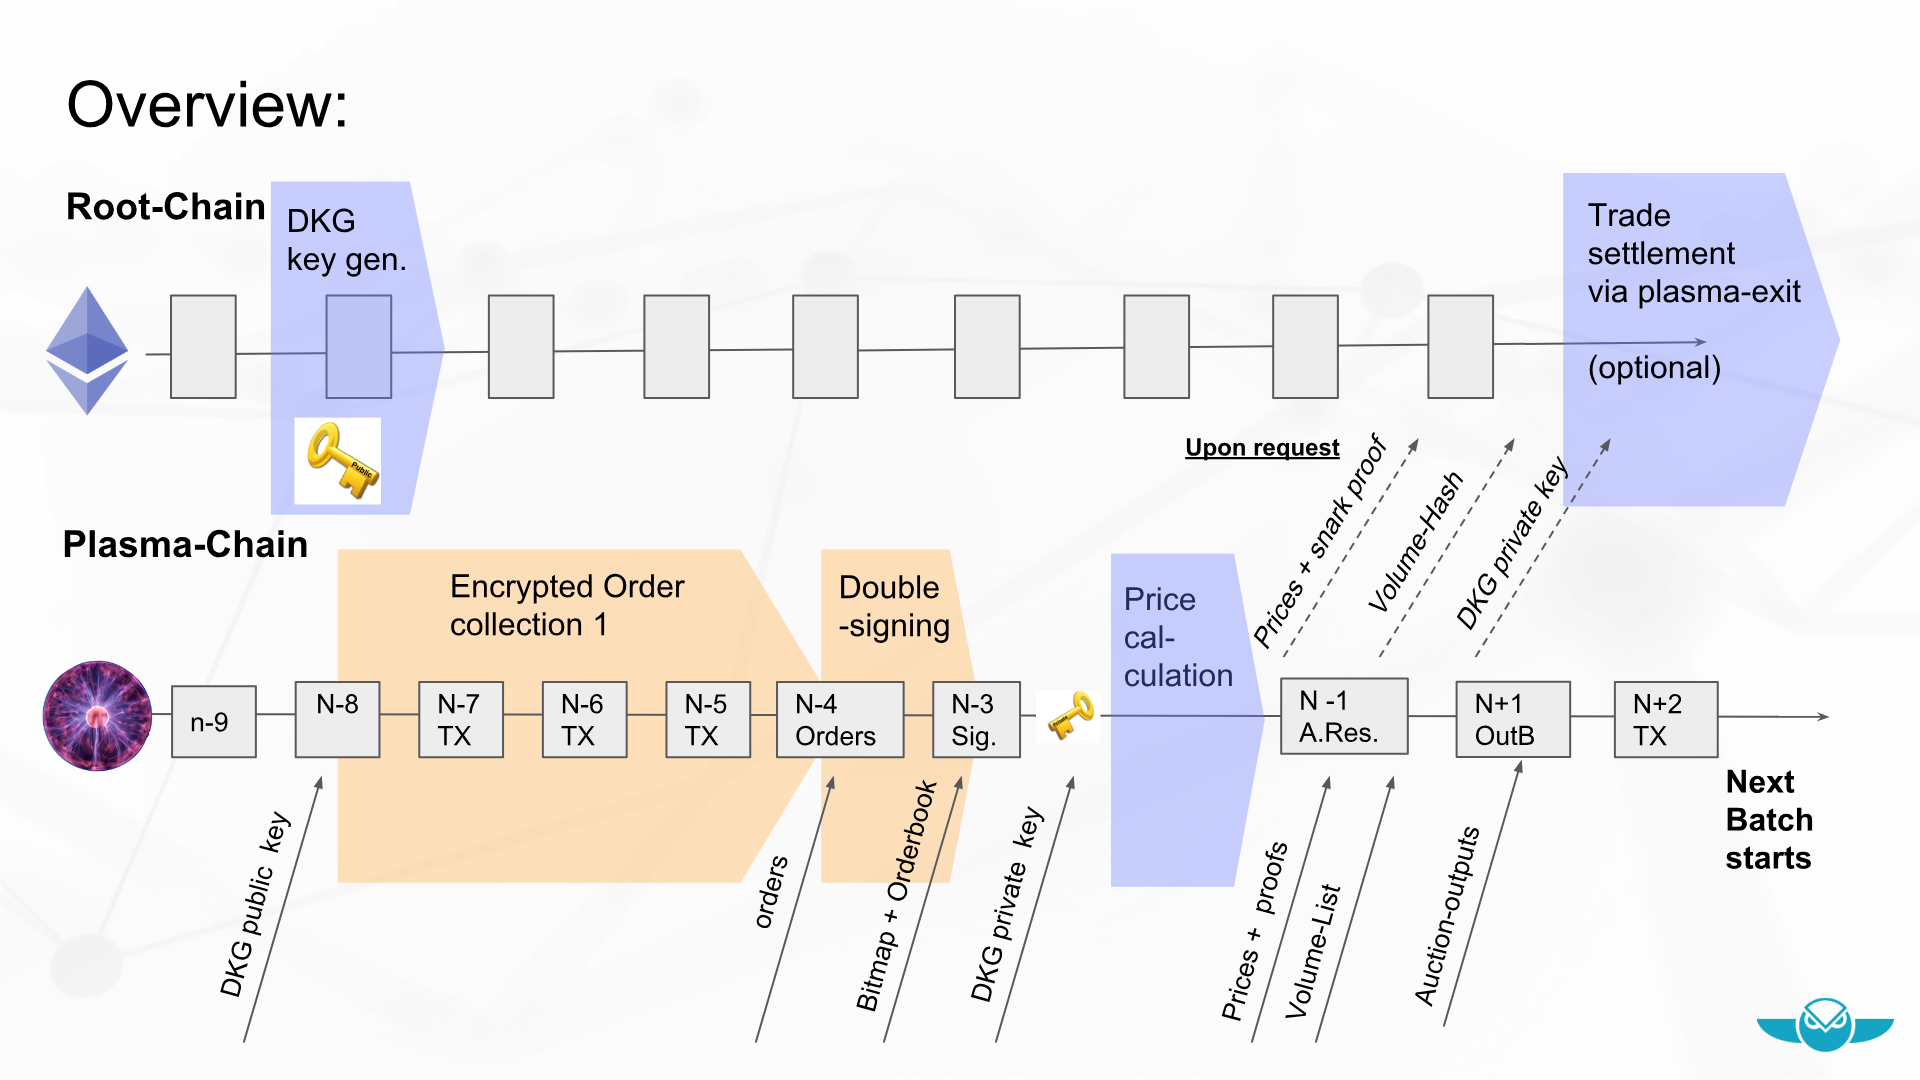
\includegraphics[width=\textwidth]{overview_tradeflow.png}
\end{figure}



\subsubsection{Encryption Key Generation}
All orders will be encrypted with a public key generated by the Distributed Key Generation (DKG) algorithm \cite{DKG}. 
A predefined number of bonded participants will be part of the DKG algorithm. 
By exchanging special messages and withholding others, they will generate a new public key for which the private decryption key is not known to any single participant. 
Only later, after the auction closes, the DKG participants are requested to publish their private messages for the generation of the private key for the decryption of the orders.
If a predefined threshold of participants publish it, this will allow anyone to generate the private key. 
If the participants publish their messages previous to the closing of the batch and its documentation on the root-chain, the protocol will allow to slashed them. 
With this approach, we have encrypted orders, unless a large portion of bonded DKG participants are malicious. 

The DKG algorithm generates a public key represented as an elliptic point $aG\label{public key}$, for a generator G of a elliptic group and a secret $a\in \mathbb{N}$ (cp. \cite{DKG}). 
This public key can then be used to encrypt messages via the ECIES \cite{ECIES}. 
Each trader calculates $bG \label{salt}$ for a random natural number b and publishes the point $bG$  in his order. 
Then he calculates: $baG$ and determines from this number the symmetric key pair for encrypting his order. 
A good symmetric encryption mechanism might be the Knudsen-Nyberg cipher\cite{cipher}, as this one would be efficient to calculate and verify using snarks in the price correctness proof \ref{proofprices}.
Later, once $a$ is public, we can decrypt the orders by calculating the symmetric key pair from $abG$, which equals $baG$. 


\subsubsection{Order Collection}
\label{orderblock}
Once the public key for the encryption process is available, every trader can submit orders. 
In the plasma chain, all assets of the ERC20 tokens are represented by unspent transaction outputs (utxo). 
An order $\pO_{i\ra j}$ will refer to a utxo of an \erc token $\tau_i$ and this utxo will be exchanged for the specified target token $\tau_j$ for a price below the given limit price. The target token and the limit price will be encrypted.

\begin{verbatim}
Order [utxo, Encry(Token j), Encry(LimitPrice), EncryptionSalt, Signatures]
\end{verbatim} 

The encryption salt is the elliptic point used for encryption:  $bG$ (cp. \ref{salt}). 
All orders will be collected and boardcast in one block per auction, the \emph{order-block}. 
All orders included in this order-block will be able to participate in the next auction. 
Theoretically, the plasma operator could censor orders, but since they are encrypted, no meaningful information could be obtained.
However, due to storage constraints (i.e. no more than $2^{16}$ orders per auction), the operator would be required to monitor the number of orders at any given time.
In the case that a participant seeks to cancel their order, they can notify the plasma operator or simply not double sign their order. 

\subsubsection{Double Signing}
Once the order-block is published and the Merkleroot hash is submitted to the root-chain, every participant in the batch auction must validate the current state of the system. 
Once they commit that their order should be included in the next batch, they will be able to withdraw their order funds only with the priority\footnote{The priority-queue is an important concept in the plasma MVP} of this order-block - this will be explained in detail here: \ref{exitRules}.

If participants validated the whole chain, they can send the operator the double signing message to signal their desire to participate. 
\begin{verbatim}
DoubleSign [OrderHash, OrderbookBlockHash, BatchIndex, Signature]
\end{verbatim}

The operator collects all these DoubleSign messages and constructs a \emph{bitmap}, in order to generate a crypto-economic signature aggregation (cp.\cite{sig}). 
The $i^{th}$ bit of this map is equal to 1 if the operator receives a DoubleSign message for the $i^{th}$ order, and is 0 otherwise.
The operator then publishes this bitmap along with all DoubleSign messages in a next plasma block. We will refer to this block as the \emph{confirmation-block}.\newline
In the event that the bitmap is unavailable or incorrect, anyone may request the operator to publish it on the root-chain, then each bit of the map could be challenged by asking the anyone to show the DoubleSign message and its Merkle-proof. 

Any unexecuted orders on this exchange will be free of charge. \todo{longterm a fee would be better... Reconsider this design choice} 
If participants take advantage of this feature to spam the plasma chain, they will be censored by the plasma plasma operator.
The operator could continue censoring their data, and this would inevitably force a spammer to withdraw their funds from the exchange.

It is clear that the process of double signing will hinder the user experience (since users would have to remain online for the duration of the auction an then act again). 
However, the possibility of granting allowance to a third-party service could be available if desired.
This would, of course, involve some level of trust in the service, but this would be limited, as this service would not be capable of altering an order. That is to say, the service would only be granted permission to double sign.

\subsubsection{DKG Private Key Generation}
Once the plasma block, containing the bitmap is published and submitted to the root-chain, the DKG participants will publish their hidden messages used for generating the DKG-public key. 
Once the threshold for the private key generation is reached and there are enough messages available to generate it, this will be published in the next plasma block by the plasma operator. 

\subsubsection{Price Submission}
Upon publication of the batch auction's private key, the operator may proceed in trying to find of the optimal price-matrix between all \erc tokens from the current batch of orders. 
While trying to find the optimal solution, we are also calculating lower and upper bounds for the solutions. Once the difference between the upper and lower bounds is small enough the operator will stop the calculation and publish the uniform cleaning prices.
As stated in before, the uniform clearing prices $\{p_{ij}| \tau_i, \tau_j \in \Tau \}$  must satisfy following equation of \emph{arbitrage-freeness} 
\begin{equation}\label{arbitrage_freeness}
p_{ij} \cdot p_{jk} = p_{ik}
\end{equation}
\begin{equation}\label{symmetric_pricing}
p_{ij} = p_{ji}^{-1}
\end{equation}
Furthermore, it is because of this constraint that it suffices for the operator to publish only the $n=|\Tau|$ prices $\{p_{ij}| \tau_j \in \Tau \}$ for some fixed (reference) token $ \tau_i \in \Tau$ and all other prices are implied.
\/* 
\begin{lemma}
Any price matrix $P = [p_{ij}]$ subject to the constraint \ref{arbitrage_freeness} of arbitrage-freeness is enjoys the following properties;
\begin{itemize}
\item[(i)] $P$ is multiplicatively-symmetric\footnote{i.e. $P^\dagger = \frac{1}{P}$ where $P^\dagger$ denotes the point-wise transpose}. Equivalently, this the result of equation \ref{symmetric_pricing}.
\item[(ii)] The diagonal of $P$ consists entirely of 1's.
\item[(iii)]  $P$ is uniquely determined by its super-diagonal entries $\{p_{i, i+1}\}_{i=1}^{n-1}$.
\end{itemize}
\end{lemma}
*/
Along with the $n-1$ price entries, the operator would publish another block consisting of a list of tuples representing order-volume pairs, 
\[[(\sigma_1, \nu_1), (\sigma_2,  \nu_2), \dots, (\sigma_N, \nu_N)]\]
where $(\sigma_i, \nu_i)$ denotes the $i^{th}$ order along with the volume $\nu_i$ of fulfilment and $N$ is the number of orders in the batch. 
This block will be referred to as the \emph{volume-block}\label{volumeBlock}

Note that, not every order below the limit price will be completely executed, the trading volume must be specified for each order.
This may come across as non-intuitive but does occur in batch auction trading.

\subsection*{3rd Party Price Submission [Optional]}
\label{publicPrices}
Usually the price would be submitted by the plasma operator only. 
But if the plasma operator does not publish the prices, we could accept price submission root-chain by any person. 
The smart contract on the root-chain would select the price submission as the final price, which is valid, has a snark valid proof of correctness and fairness and has the biggest trading volume measured in Ether. 

Note that in this case, the price submitter would also need to provide the volume-block (cp. \ref{volumeBlock}) or at least assist traders with their exits games, by providing the Merkle proofs for their trading volumes (cp. \ref{exitRules}). 

\subsubsection{Proof of Correctness and Fairness}
\label{proofprices}
Once the prices are calculated by the plasma operator, he needs to prove that this set of prices is actually valid and fair. A price set and a volume-block (VB) \ref{volumeBlock} is valid and fair, if

\begin{itemize}

\item the price set satisfies \ref{eq:arbitrage_freeness} 
\item Orders are only touched, if the limit price is below the calculated price:\newline
\begin{equation} \forall \tau_i ,\tau_j \in \Tau \quad \forall \sigma \in \pO_{i\ra j}, \quad \nu_{p_{ij}}(\sigma)>0 \Rightarrow p_{ij}\geq \text{p}(\sigma)
\end{equation}
\item the amount of sell volume for a token equals its buy volume: 
\begin{equation}
\begin{split}
\forall \tau_i \in \Tau \quad \sum_{\tau_j\in \Tau} \,
\sum_{ \sigma\in \pO_{i \rightarrow j}} \nu_{p_{ij}}(\sigma) = \sum_{\tau_j\in \Tau} \, \sum_{\sigma\in \pO_{j\rightarrow i}} \frac{\nu_{p_{ji}}(\sigma)}{p_{ji}}
\end{split}
\end{equation}
\item If an order $\sigma \in \pO_{i\rightarrow j}$ with a limit price p has a positive trading volume, then every order in $\pO_{(\tau_i\rightarrow \tau_j)}$ with a lower limit price should be completely fulfilled. 
\end{itemize}


In order to prove this, we will use snarks (succinct non-interactive arguments of knowledge) \cite{snarks}. 
In brief, snarks are a powerful tool enabling us to encode the above mentioned check-logic as an algebraical formulation. 
%This allows us to generate some verification keys, which compactify this checking logic. 
Then for each set of prices and any volume-block, one can quickly generate a proof that the above constraints are satisfied using verification keys. 
The proof size is very small (8 variables of type bytes64) and can easily be provided to the root-chain. 
It turns out that the execution of such a proof would cost approximately1.6 million gas on the root-chain. 
The library ZoKrates \cite{zokrates} demonstrates these methods very well within the ethereum eco-system. 

\subsection*{An elaboration on the snark mechanism}
Let $\mathcal{B}_O$, $\mathcal{B}_V$ and $\beta$ denote the order-block, volume-block and bitmap introduced above (respectively). 
In the following we denote the block containing all orders OB\ref{orderblock}, the volume-block VB \ref{volumeBlock}, the bitmap B and $M_R(OB)$, $M_R(VB)$, $M_R(B)$ their Merkleroot hashes, respectively.
Let us denote the decrypted orders from the block OB as list $\text{[orders]= [order}_1\text{, order}_2\text{,...]}$ and the trading volume of each order by the list $\text{[volumes] = [volume}_1\text{, volume}_2\text{...]}$, where the $\text{volume}_i$ corresponds to the $\text{order}_i$. 


Then the program P(i,w) should prove the above mentioned facts. 
The public input into P is declared by the variable i and w will be the witness. 
In details it will look like:

\begin{equation}
\text{P(i=(}M_R\text{(OB),}M_R\text{(VB),}M_R\text{(B),} \text{key}_p),\newline
\text{w=([orders],[volumes],[prices],[bitmap]))} 
\end{equation}
And P would check that:
\begin{itemize}
\item  $M_R(\text{OB}) == M_R(\text{Encrypted[orders]})$
\item  $M_R(\text{VB}) == M_R(\text{[orders]} \cup \text{[volumes]})$,\newline
where $\text{[orders]} \cup \text{[volumes]} = \text{[order}_1, \text{volume}_1, ...] $
\item $ M_R(\text{B}) == M_R(\text{[bitmap]})$
\item $\forall o \in \text{[orders], vol}(o)>0 \implies \text{bitmap}(o) = 1 $, 

\item 
\begin{equation}  \forall \tau_i ,\tau_j \in \Tau \quad \forall o \in \pO_{i\ra j}, \quad \nu_{p_{ij}}(o)>0 \Rightarrow p_{ij}\geq \text{p}(o)
\end{equation}
\item 
\begin{equation}
\begin{split}
\forall \tau_i \in \Tau \quad \sum_{\tau_j\in \Tau} \,
\sum_{ o\in \pO_{(\tau_i \rightarrow \tau_j)}} \nu_{p_{ij}}(o) == \sum_{\tau_j\in \Tau} \, \sum_{o\in \pO_{(\tau_j\rightarrow \tau_i)}} \frac{\nu_{p_{ji}}(o)}{p_{ji}}
\end{split}
\end{equation}
\item For each trading pair, P loops through all orders and memorizes the highest limit price of an order of this pair, which still has a positive trading volume. 
Then it loops through them again and checks that no other order with a lower limit price has not been filled. 
\end{itemize}

Once the proof is calculated, the plasma operator will publish it on the plasma chain. 


\subsubsection{Enforcing Key Variable Publication}

\label{enforceAvailablity}
In case the operator goes off-line and we get a data-unavailability, we still want to make sure that the last auction can be completed by all participants or it will be cleanly un-rolled. 
Since data-availability on the plasma chain is subjective, we need to make sure that all necessary information will be loaded into the root-chain, in the worst case. 
The necessary data is the bitmap ($2^{16}$ bits), the private key for decrypting the orders (2x $32$ bytes), the prices (n x $32$ bytes) and the proof for correct volumes (10 x $32$ bytes).

\paragraph{bitmap}
It is essential for everyone to know, what the bitmap of an auction is, in order to know which orders are in the batch. 
If the bitmap has not been sent out by the plasma operator, we have to make it available on the root chain. 
Everyone can request - in exchange for a small fee - that the bitmap gets published on the root chain. 
Then anyone can publish the bitmap along with a plasma containment proof of this bitmap and get the fee. 
If no one publishes it, then the last batch will be rolled back completely. 
This means that only utxos, which were submitted before the last order book hash submission, will be accepted for any withdraw. 

\paragraph{decryption keys}
Also, the decryption key of an auction is essential to know, in order to see the limit prices of the encrypted orders. 
If the decryption key is not publicly available, we can apply the same process as for the bitmap to make it public. 

\paragraph{prices}
The prices are also essential to know for each participant. 
If they are not public, again they can be made public with the same mechanism. 
We note that the gas costs for publishing the prices increase linearly with the number of tokens. 

\paragraph{price verification}
The proof of the correctness is initially only stored in the plasma chain. 
But anyone can request to publish the proof also on the root-chain. 
We use again the same mechanism as before. 


\subsubsection{Order-output Transactions}
After the prices and a price verification proof are published, the operator will publish another block with all order-output transactions. 
An order-output transaction for an order within $\pO_{i\ra j}$ will have the following format:

\begin{lstlisting}
OrderOutput [ Order txHash,
    Order output denominated in Token $\tau_j$ ($oo_j$), 
    newOwner,
    Order output denominated in Token $\tau_i$ ($oo_i$),
    orderCreator]

\end{lstlisting}
where the order-output denominated in Token $\tau_i$ should be zero is the most cases, as orders will be most likely be fully filled. 
The order-output ($oo_j$) denominated in Token $\tau_j$ will be calculated by the price 
\begin{equation}
  oo_j = p_{ij} \times \text{OrderInputAmount} \times \nu(\text{order}) \times (1-\text{fee}_{\text{ratio}})
    \label{fee_equ}
\end{equation}
where $\nu(\text{order})$ is the volume declared in the volume-block.  
Whereas, the order-output ($oo_i$) denominated in Token $\tau_i$ is simply the left over, if the trade could not be executed completely: 
\begin{equation}
  oo_i =  \text{OrderInputAmount} - \nu(\text{order})
\end{equation}
These order-outputs can then be spent again via a transaction, but cannot be used as an input for another order. 
If any of these order-outputs is not correctly created by the plasma operator, people have to leave the plasma chain. 
Then the last batch will be settled on the root-chain or be reverted, depending whether all trading volumes are available. 

\subsubsection{Claiming Fees}
After each batch auction, the plasma-contract on the root-chain will hold some tokens, which are not covered by transaction outputs in the plasma chain, due to fee mechanism specified in \ref{fee_equ}. 
The plasma operator is allowed to create a new utxo with the number of uncovered tokens, in order to claim the fees. 

\subsubsection{Auction scheduling process}

An auction can have a variable timing. 
The operator can decide on his own when to close the batch and create the order-block \ref{orderblock}. 
Once this block is posted, it will take some time until the orders are processed. 
But the operator will ensure a smooth flow by accepting new orders right away. 
But of course, these orders and all transfers will not be executed if the chain will halt. 
Hence batch auctions can be scheduled pretty fast and smooth one after the other. 
But the finality of an auction is only guaranteed after the client sees all the data available for a batch auction, including the bitmap, decryption key, prices, and price verification data. 


\subsection{Exit rules of the plasma chain}
\label{exitRules}
\paragraph{Transfer transactions} have quite the same exit rules, as in the usual plasma mvp. 
But there are two differences.
\begin{itemize}

 \item We would maintain a variable \emph{highestExitPriority}. 
This highestExitPriority would be infinity in normal cases. 
But if the plasma chain is halted, because a data-unavailability request \ref{enforceAvailablity} was not answered in a certain time frame, then this variable will play an important role. 
It will set the highest exit priority to the priority of the last block, before the order-block submission. 
Any utxo generated after highestExitPriority will not be exitable and any exit request cannot be challenged with a utxo spend after this highestExitPriority. 
Effectively, we are resetting the plasma state to a previous state by setting highestExitPriority. 
\item Any utxo can be challenged as spent and not exit-able, by showing an order, a double signing of the order and that the trading volume of this order is positive. Of course the Merkle proofs for this data needs to be provided.

\end{itemize}

\paragraph{Order transactions} can also be referenced for an exit request. The request are put into the same priority queue as the normal exits. They need to prove that the order transaction was also double signed and had a positive trading volume by providing data by providing Merkle proofs for it.
For a "touched" order in $\pO_{i\ra j}$ only the target token $\tau_j$ can be withdrawn, but not the input token $\tau_i$. 
Hence, trades are enforced and cannot be reverted arbitrarily. 
If a data-unavailability appears right after the closing the batch, the order-output transaction might be already in a plasma block. 
These order-outputs cannot be used to challenge an order exit. 
Only if the order-output is already spent and double signed, then the order exit process can be challenged successfully. 
It might happen that a trader does not know the trading volume of his order in the last batch auction because the order-output block might be unavailable for him. 
Then, he would not be able to provide the Merkle proof to attest his positive trading volume. 
In this case, we would ask on anyone to complete his exit, by providing the Merkle proof with the trading volume. 
If neither the plasma operator nor anyone else does answer this exit request within 7 days, then the auction will be stopped and all trades will be reverted if the auction was conducted in the last 7 days. If the auction was not conducted in the last 7 days, then the exit requester should have the data available.


\newpage

\section{Features}

\subsection{Trade enforcement}
Trades on this exchange will usually be enforced. 
That is, if an order was submitted, double signed and was touched by auction price, then the actor can only withdraw the trade-output nominated in the target token. 
But the trader will not back his trade input. 

Unfortunately, some actors have an advantage.
If many DKG key holders do not reveal the decryption key, they can stop the chain. 
The DKG algorithm works with a predefined threshold. 
Only if more DKG participants as specified by the algorithm do not reveal their private input, then the batch cannot be executed. 
But in this case, we could also slash these DGK participants, which are misbehaving. 

\subsection{Safety in case of a data-unavailability}
For token transfers, we have the same data-unavailability fallbacks, as the MVP product. 
Hence a double sign mechanism protects people from losing funds. 
It is only getting a little bit more complex, as users should not double sign a transaction, which happens right after the closing of a batch, before they validated the WHOLE process of the batch closing, including the publishing of valid prices, snark proofs of correctness and a correct order-output block. \newline
Also for traders, the safety is guaranteed by a  double signing mechanism. 
If there is anything incorrect, before the double signing step, traders will just not double sign their batch. 
If any network attack happens right after the order block, the traders withdrawal priority will still be higher than any withdrawal request of this attack. Hence traders will always get their funds back or they can settle the last batch via the on chain exit. 
If there is any data not available for settling the trade with an exit request after the double signing step, then this data can be requested to be uploaded to the root chain. 
The exchange is constructed in such a way with snarks and bitmaps, that it is easy and relatively cheap to publish this data on the root-chain. 
If the data is published, any trader can get his trade settled on chain. If the data is not published, the batch is reverted. 
For a detailed description of the data, which needs to be made available, see here: \ref{enforceAvailablity}. 
The proof that this data is enough to settle the trade either on the plasma chain or on the root-chain is left to the reader. 

\subsection{Non-custody of funds}
From the above analysis, we can conclude that the plasma plasma operator does never have the ability to steal tokens if all users come online regularly and behave correctly. 
This is one of the key features of this construction. 

\subsection{Grieving vectors and tragedy of the common}
Unfortunately, our specification had to take some trade-offs. 
The main problem is that data-unavailability is subjective. 
Hence, people can always claim that data is missing. 
Then someone is required to publish these data on the root-chain including a Merkle proof attesting that the published data is the same as on the plasma chain. 
This is a problem, since providing data on the root-chain can be quite costly. 
Our solution is that the requester needs to pay some decent fee to the data-provider, in order to prevent grieving attacks. 
But this leaves the construction with a tragedy of the commons, as no one, in particular, would have the incentive to ask for the data in case of a real data-unavailability case. 
But still, this action would be required from someone. 

Since we estimate the costs of this data-request on the root chain to be definitively lower than 10 Dollar, the tragedy of the commons is very small. 
There should always be a party, which request the data for everyone else. Hence, it is a reasonable trade-off. 

Since the plasma plasma operator will never intentionally generate these situations, as it will hurt his reputation, the incentives are well set. 

\subsection{Performance}
There are some bottlenecks, which are considered for evaluating the performance:
\begin{itemize}
\item Price calculation. 
Finding these uniform clearing prices is a non-linear optimization problem. 
The solving time to find these prices increases exponentially with the number of tokens involved. For concrete timings, take a look at this paper \cite{priceOptimization}
\item Generating the public verification keys for the snark proofs is a very challenging task having its own limitations. 
But we think that we can generate these verification keys for trade blocks with $2^{16}$ transactions. 
The calculation of the actual proof should then be feasible within a minute. 
\item Gas costs for bitmap and other data, which needs to be made available on the root-chain. 
Uploading a bitmap with 9000 entries costs about 100k gas. 
\item Plasma exists.
Plasma exits are controversially discussed in the community. 
If there are too many utxo, which want to exit all at the same time, - maybe triggered by a data-unavailability -, the root chain will be under heavy load and gas prices might spike. 
\end{itemize}
We think that the price calculation is the biggest bottleneck. 
But still, we are confident that we will be able to schedule auctions every 3 minutes with about $2^{16}$ orders. 
\subsection{Complexity}
Unfortunately, the described mechanisms are quite complex. 
Shipping such a complex construction without any bugs will require a huge engineering effort. 
Hence, Gnosis is planning to cut out some features and add them only in the next versions of its product. 

The following pieces can reduce the complexity:
\begin{enumerate}
\item
DKG can be replaced with one single entity, which is very trustworthy. 
This single entity would only generate the public keys and later reveal the private keys for it. 
This does not put customers funds at risk at any point in time. 
\item
The described mechanism \ref{publicPrices} making it possible to everyone to submit the best prices can be left out. 
\end{enumerate}

\section{Open research questions}

\subsection{Future iterations}
We hope that in future iterations, we can outsource more and more logic to the snarks proofs. 
This has the potential to improve the user experience a lot since verification times will be reduced and double signing processes can be omitted. 

\subsection{Plasma rollovers}
In order to reduce the verification time for clients, a potential solution is a chain rollover. 
That is, all transaction outputs needs to be spend all 3 weeks. 
If people do not send them to themselves within 3 weeks, they will not longer be exit-able from the plasma chain. 
In a plasma chain, where transactions are for free, this is a viable model. 
It does not really come with any new burdens for the users, as the user needs to be online and check the validity of the chain anyways.

But it would have the big benefit that not the whole chain needs to be stored and processed, but only the blocks of the last 3 weeks. 

\begin{thebibliography}{9}
\bibitem{DKG} 
Caimu Tang
\textit{ECDKG: A Distributed Key Generation Protocol Based on Elliptic
Curve Discrete Logarithm.}  
https://pdfs.semanticscholar.org/3c52/35523be1d305de6dbf3433965c99d9fe4aea.pdf
 

\bibitem{priceOptimization} 
Gnosis
\textit{Multi-token Batch auctions with uniform clearning prices}  
https://github.com/gnosis/dex-research/tree/master/BatchAuctionOptimization

\bibitem{plasma} 
Vitalik Buterin and Joseph Poon
\textit{Plasma}.
https://plasma.io/plasma.pdf

\bibitem{MVP} 
Vitalik Buterin
\textit{Plasma minimal viable product}.
https://ethresear.ch/t/minimal-viable-plasma/426
 
\bibitem{sig} 
Crypto aggregated signatures
\\\texttt{}
https://ethresear.ch/t/cryptoeconomic-signature-aggregation/1659

\bibitem{snarks} 
Snarks using the library Zokrates
\\\texttt{snarks}

\bibitem{ECIES} 
ECIES
\\\texttt{ECIES}
https://crypto.stackexchange.com/questions/31602/how-does-encryption-work-in-elliptic-curve-cryptography

\bibitem{cipher} 
Knudsen-Nyberg cipher
\\\texttt{ Knudsen-Nyberg cipher}
https://eprint.iacr.org/2016/492.pdf


\bibitem{batch} 
Batch Trading - \href{https://www.investopedia.com/terms/b/batchtrading.asp}{https://www.investopedia.com/terms/b/batchtrading.asp}

\bibitem{zokrates} Snarks - \href{https://github.com/JacobEberhardt/ZoKrates}{https://github.com/JacobEberhardt/ZoKrates}

\end{thebibliography}

\end{document}
